\documentclass{standalone}

\usepackage{tikz}
\newcommand\fl[1]{\texttt{#1}}
\usetikzlibrary{decorations.markings}
\tikzset{->-/.style={postaction=decorate,decoration={markings, mark=at position
#1 with \arrow{latex}}}}

\begin{document}
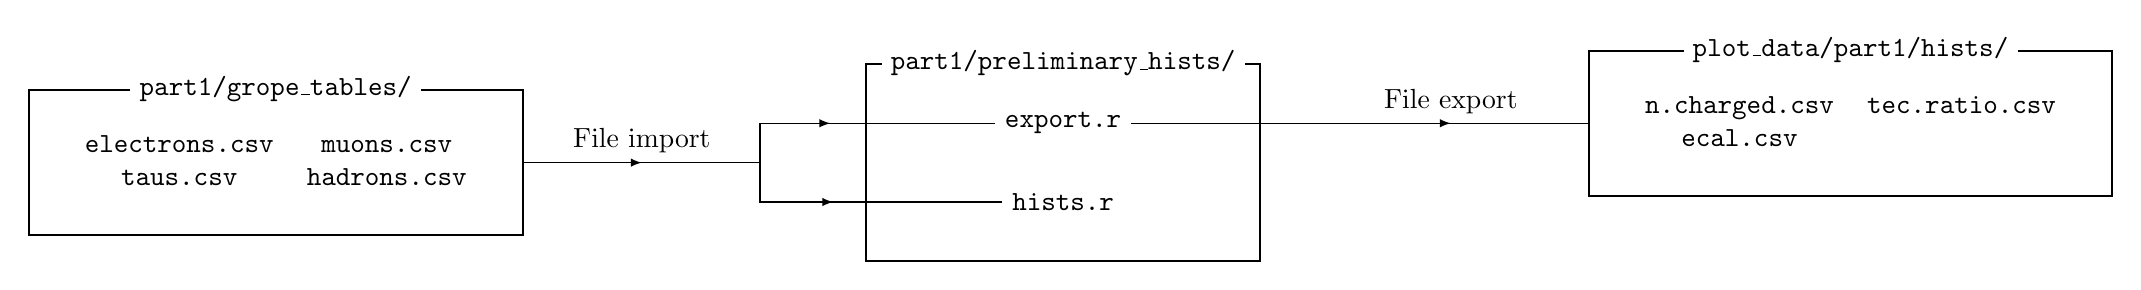
\begin{tikzpicture}
  \node[draw, thick, inner sep=.5cm] at (0, -.5) (in){%
    \begin{tabular}{cc}
      \fl{electrons.csv} & \fl{muons.csv} \\
      \fl{taus.csv} & \fl{hadrons.csv} \\
    \end{tabular}
  };
  \node[fill=white] at (in.north) {\fl{part1/grope\_tables/}};

  \node[draw, thick, minimum height=2.5cm, minimum width=5cm, inner sep=.5cm] 
    at (10, -.5) (eval) {};
  \node[fill=white] at (eval.north) {\fl{part1/preliminary\_hists/}};
  \node (hists) at (10, -1) {\fl{hists.r}};
  \node (export) at (10, 0) {\fl{export.r}};

  \draw[->-=.5] (in.east) --++ (3, 0) coordinate(temp)
    node[midway, above]{File import};
  \draw[->-=.40] (temp) |- (hists);
  \draw[->-=.4] (temp) |- (export);

  \node[draw, thick, inner sep=.5cm] at (20, 0) (out){%
    \begin{tabular}{cc}
      \fl{n.charged.csv} & \fl{tec.ratio.csv} \\
      \fl{ecal.csv} & \\
    \end{tabular}
  };
  \node[fill=white] at (out.north) {\fl{plot\_data/part1/hists/}};

  \draw[->-=.7] (export) -- (out.west) node[pos=.7, above]{File export};
\end{tikzpicture}
\end{document}
